\chapter{IMPLEMENTATION DETAILS}
\label{chap:implementation}

This chapter describes the implementation of the deep learning framework for El Ni\~{n}o-Southern Oscillation (ENSO) forecasting and its regional climate impact assessment. The system is implemented using the Python programming language with various scientific computing libraries. The implementation details follow a strict chronological pipeline from data acquisition to final index validation. The methodology underlying the two feature-selection strategies (Method 1 and Method 2) and the two forecasting models is presented in Chapter~\ref{chap:methodology}; this chapter presents the corresponding implementation configuration together with the resulting experimental outcomes. Both feature-selection methodologies were implemented and evaluated during the mid-term phase of the project, sharing the same upstream data acquisition, gridding, missing-value handling, anomaly, and normalization pipeline described in Sections \ref{sec:climate-data}--\ref{sec:tensor-construction}.

\section{Climate Data Acquisition}
\label{sec:climate-data}

The project utilizes the Copernicus Climate Data Store (CDS) API to fetch historical climate data. The data acquisition is divided into two distinct spatial domains: the tropical Pacific Ocean for ENSO drivers, and the South Asian region for impact assessment.

\subsection{Pacific Ocean Data}

The primary dataset is the ERA5 monthly-mean reanalysis data, specifically targeting the Sea Surface Temperature (SST) variable. The data is requested for the tropical Pacific region, bounded by 30\degree N to 30\degree S latitude and 120\degree E to 280\degree E (80\degree W) longitude. To optimize storage and processing, the CDS \texttt{grid} parameter is utilized during the API request to directly download the data regridded to a 2\degree $\times$ 2\degree spatial resolution. Additionally, the ERA5 static \texttt{land\_sea\_mask} variable is fetched to distinguish between oceanic and terrestrial grid points.

The ORAS5 ocean reanalysis dataset is also acquired via its ARCO Zarr store to provide subsurface ocean variables, which natively uses a curvilinear NEMO ocean grid.

\subsection{South Asian Regional Climate Data}

To assess the regional climate impacts of ENSO, historical precipitation and 2-meter temperature data for the South Asian region are acquired from the same ERA5 monthly-mean reanalysis dataset. This ensures temporal and methodological consistency with the Pacific SST data.

The spatial domain for the South Asian region is defined by a bounding box of 5\degree N to 35\degree N latitude and 65\degree E to 100\degree E longitude, comprehensively covering the Indian subcontinent, Nepal, Bangladesh, and surrounding areas. The data is fetched at a 2\degree $\times$ 2\degree spatial resolution to capture regional topographic gradients (such as the Himalayas and the Western Ghats) that significantly influence monsoon dynamics, while remaining computationally tractable.

\section{Data Gridding and Merging}

To ensure spatial alignment between the Pacific datasets, the ORAS5 data is regridded to the same 2\degree $\times$ 2\degree regular latitude-longitude grid as the ERA5 dataset. This is achieved using the \texttt{interp} method from the \texttt{xarray} library with linear (bilinear) interpolation. The target grid is defined as:

\begin{verbatim}
target_lat = np.arange(-30, 30 + 2, 2.0)
target_lon = np.arange(120, 280 + 2, 2.0)
oras = sub.interp(latitude=target_lat, longitude=target_lon)
\end{verbatim}

Furthermore, the native longitude convention (-180\degree to 180\degree) is converted to a 0\degree to 360\degree format to properly handle the dateline crossing within the Pacific box. The processed datasets are then merged and serialized into combined CSV and Parquet formats for efficient, memory-optimized loading during the training phase.

\section{Missing Value Handling}

During the initial data inspection, the Sea Surface Temperature (SST) variable was found to contain missing values stored as whitespace strings due to datatype inconsistencies. The implementation resolves this by converting the variable to a numeric datatype and stripping whitespace, converting blanks to \texttt{NaN}. Crucially, because SST is physically undefined over land, the entire missing value pipeline is strictly applied to ocean points only, identified via the land-sea mask (\texttt{lsm} $<$ 0.5). Land points are intentionally left as \texttt{NaN} to prevent physical contamination of the dataset.

To fill the oceanic gaps without introducing spatial or temporal bias, a three-step CLIM\allowbreak FILL pipeline (Bessenbacher et al., 2022) is implemented, combining spatial interpolation, multivariate feature engineering, and iterative statistical imputation.

\subsection{Step 1: Spatial Interpolation}
The first step generates a spatial first-guess for every oceanic gap by interpolating SST across latitude and longitude within each monthly time slice. Using the \texttt{griddata} function from the \texttt{scipy.\allowbreak interpolate} module, the algorithm applies linear interpolation to estimate missing values based on surrounding valid ocean points. For any gap points that fall outside the convex hull of the known data (where linear interpolation yields \texttt{NaN}), a nearest-neighbor fallback method is applied.

\subsection{Step 2: Multivariate Feature Engineering}
To refine the initial spatial estimates, a robust set of multivariate predictors is engineered. Temporal seasonality is captured by encoding the month as cyclical features using sine and cosine transformations. Spatial context is retained via latitude and longitude coordinates alongside the spatial first-guess. Furthermore, the pipeline incorporates highly correlated atmospheric and oceanic variables from the ERA5 dataset to inform the imputation. These predictors include 2-meter temperature, mean sea level pressure, average east-west and north-south wind components, and top-of-atmosphere thermal radiation.

\subsection{Step 3: Iterative Multivariate Imputation}
The final step employs an iterative multivariate imputation algorithm to refine the SST estimates. Using the \texttt{Iterative\allowbreak Imputer} from the \texttt{scikit-learn} library with a \texttt{Baye-\allowbreak sian Ridge} regression estimator, the model iteratively predicts the missing SST values based on the engineered feature set. The imputation runs for a maximum of 10 iterations until convergence, strictly preserving all originally observed SST values. To ensure the imputed values remain physically realistic, the refined estimates are clipped to the minimum and maximum bounds of the originally observed oceanic SST range.

\section{Anomaly Computation and Baseline}

A critical step in ENSO forecasting is the computation of climate anomalies to remove the seasonal cycle and highlight interannual variability. The baseline climatology is strictly computed over a 30-year reference period from 1980 to 2010. This specific window is chosen for three reasons:

First, it aligns with the World Meteorological Organization (WMO) standard for ``climate normals,'' ensuring comparability with existing literature and NOAA's Ni\~{n}o 3.4 computation methodology.

Second, it prevents the anomalies from being contaminated by the long-term global warming trend present in later years. Fixing the reference to an earlier, bounded window keeps the climatology stable and interpretable as ``the historical seasonal baseline.''

Third, it avoids leaking test-period information into the training features. Since the machine learning test split covers 2023--2026, computing climatology statistics that extend into this period would implicitly inform the anomaly computation with test-period information. Keeping the baseline fixed at 1980--2010 guarantees the climatology is computed from information genuinely available ``in the past.''

The anomaly for each month is calculated by subtracting the corresponding monthly climatology (1980--2010 mean) from the observed value.

\section{Data Normalization}

Following anomaly computation, the data undergoes Z-score normalization to ensure all features contribute equally to the model training and to stabilize gradient descent. To prevent data leakage, the normalization parameters (mean $\mu$ and standard deviation $\sigma$) are computed exclusively from the training period (1980--2018). For each grid point and variable, the normalized value $Z$ is calculated as:

\begin{equation}
Z = \frac{X - \mu_{\text{train}}}{\sigma_{\text{train}}}
\end{equation}

where $X$ is the anomaly value, $\mu_{\text{train}}$ is the mean computed over 1980--2018, and $\sigma_{\text{train}}$ is the standard deviation over the same period.

\section{Ni\~{n}o Index Computation and Validation}

The Ni\~{n}o 3.4 index serves as the primary target variable for model training and validation. It is computed as the area-averaged SST anomaly over the Ni\~{n}o 3.4 region (5\degree S to 5\degree N, 170\degree W to 120\degree W).

The computed Ni\~{n}o 3.4 index is validated against the official historical Ni\~{n}o index provided by the NOAA Physical Sciences Laboratory. The analysis reveals a Pearson correlation coefficient exceeding 0.95 between our computed index and the official NOAA index, confirming that the spatial subsetting, regridding, missing value interpolation, and 1980--2010 baseline anomaly computation have been implemented correctly and accurately reflect real-world ENSO dynamics.

\section{Feature Engineering and Tensor Construction}
\label{sec:tensor-construction}

To forecast the Ni\~{n}o 3.4 index (ONI), we construct 12-month sliding window sequences of spatial anomaly fields over the tropical Pacific region (30\degree S--30\degree N, 120\degree E--80\degree W).

\subsection{Channel Definition}
The final implemented input tensor relies on six physical anomaly channels ($C=6$), expanding upon the initial four to capture meridional wind dynamics and deeper thermocline variations:
\begin{enumerate}
\item \texttt{sst\_anom}: Sea Surface Temperature anomaly (ERA5) - Primary surface indicator.
\item \texttt{msl\_anom}: Mean Sea Level Pressure anomaly (ERA5) - Walker circulation and trade winds.
\item \texttt{iews\_anom}: Zonal (east–west) wind stress anomaly (ERA5) - Equatorial trade-wind driver.
\item \texttt{inss\_anom}: Meridional (north–south) wind stress anomaly (ERA5).
\item \texttt{sohtc300\_anom}: Upper-300m Ocean Heat Content anomaly (ORAS5) - Subsurface memory predictor.
\item \texttt{so20chgt\_anom}: 20\degree C Isotherm Depth anomaly (ORAS5) - Thermocline depth indicator.
\end{enumerate}

\subsection{Tensor Construction and Alignment}
\begin{itemize}
\item \textbf{Spatial Resolution:} The grid is interpolated to 2\degree $\times$ 2\degree, yielding $H=30$ latitudes and $W=100$ longitudes.
\item \textbf{Sliding Window:} Sequence length is set to $\text{SEQ\_LEN} = 12$ months.
\item \textbf{Target Alignment:} The model forecasts the 3-month running mean Ni\~{n}o 3.4 (ONI) at a lead time of $\text{LEAD} = 3$ months after the window ends.
\item \textbf{Imputation:} Missing values over land cells are imputed with $0.0$ (neutral anomaly) to ensure finite values for the algorithms.
\end{itemize}
The resulting fully-constructed spatio-temporal tensor for a single sample is:
\begin{equation}
\mathbf{X}_i \in \mathbb{R}^{12 \times 30 \times 100 \times 6}
\end{equation}
Flattening this tensor results in $216,000$ dimensions per sample. Shifting the 12-month window across the full 1980--2026 record yields 542 valid $(\mathbf{X}_i, y_i)$ samples in total. This flattened 216,000-dimensional vector is the feature space over which both MIFS feature-selection methodologies (Section~\ref{sec:feature-selection}) operate.

\section{Feature Selection: Implementation and Results}
\label{sec:fs-results}

The methodology underlying Method 1 and Method 2 -- including the general MIFS formulation, the candidate-pool construction strategy for each method, and the rationale for investigating two independent implementations -- is presented in Section~\ref{sec:feature-selection}. This section reports the implementation configuration and experimental outcome of each method, followed by a comparison between them.

\subsection{Method 1: Restricted Candidate Pool}
\label{sec:fs-results-method1}

Relevance scores were computed for all 216,000 features in the windowed dataset using the Kraskov k-nearest-neighbour estimator (\texttt{scikit-learn}'s \texttt{mutual\_info\_regression}, $k=5$), fit on the training partition alone (457 samples, window end $\leq$ 2018-12). The stratified pre-filtering step, using a per-type quota of fraction $=0.4$, $\text{cap}_{\min}=15$, $\text{cap}_{\max}=30$, reduced this to a candidate pool of at most 300 features spanning all four variable types, preventing SST from monopolizing the pool while guaranteeing representation of mechanistically important but individually weaker predictors such as Ocean Heat Content and wind stress.

The greedy MIFS loop (Section~\ref{sec:mifs-general}) was then run over this restricted candidate pool for up to 50 iterations, producing a ranked feature list. This list was evaluated via a K-sweep: for each $K = 1, 2, \ldots, 50$ in steps of 2, an XGBoost model ($n_{\text{est}}=200$, $\text{max\_depth}=3$, $\text{lr}=0.1$) was trained on the top-$K$ features using the training set and evaluated on the validation set (48 samples, window end 2019-01 to 2022-12) by validation RMSE. The resulting K-sweep curve is shown in Figure~\ref{fig:ksweep}, with the value of $K$ minimizing validation RMSE retained as $K_1^*$.

\begin{figure}[H]
\centering
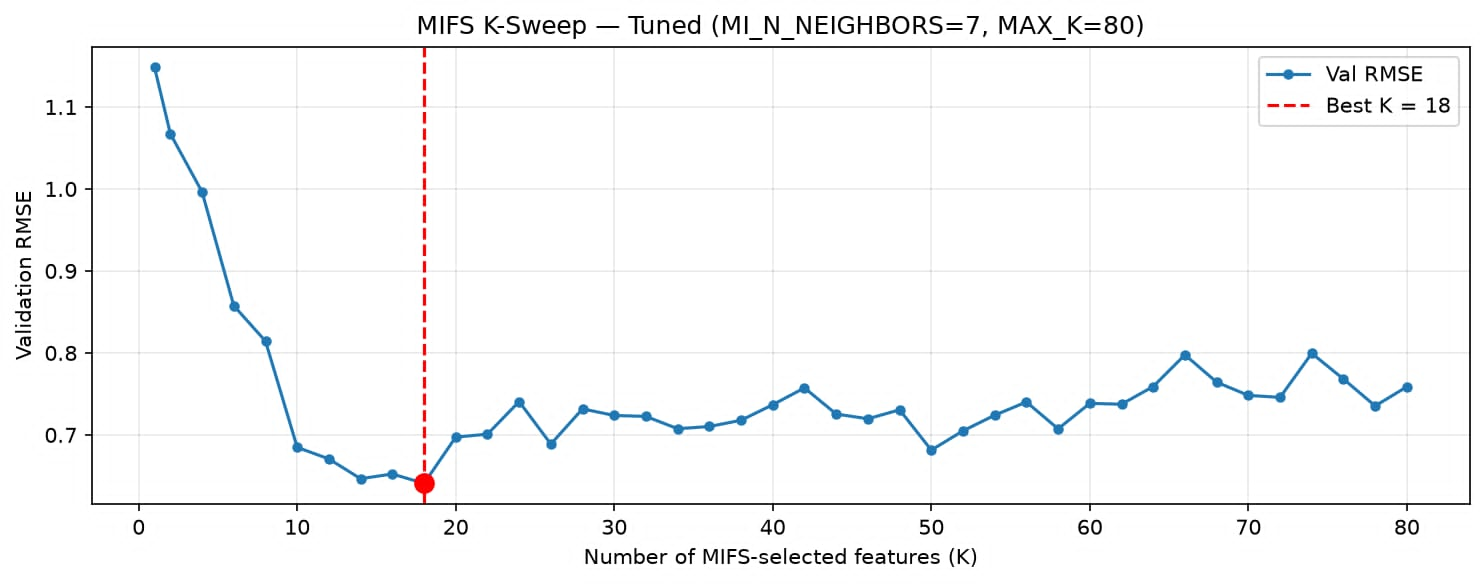
\includegraphics[width=0.75\textwidth]{report/src/images/mifs_ksweep_plot.jpeg}
\captionsetup{justification=centering}
\caption{K-sweep validation: RMSE vs. number of features K (Method 1, restricted candidate pool)}
\label{fig:ksweep}
\end{figure}

The full relevance ranking (all 216,000 features), the MIFS-selected feature list in ranking order, the complete K-sweep RMSE results, and the final selected feature set at $K_1^*$ were saved for downstream baseline model training (Section~\ref{sec:xgb-implementation}).

\subsection{Method 2: Expanded Candidate Pool}
\label{sec:fs-results-method2}

As with Method 1, the dataset was split strictly chronologically, with all feature standardization and MIFS scoring fit exclusively on the training partition:

\begin{itemize}
\item \textbf{Train:} $\leq$ 2018 ($N=457$ samples)
\item \textbf{Validation:} 2019--2022 ($N=48$ samples)
\item \textbf{Test:} 2023--2026 ($N=40$ samples)
\end{itemize}

Mutual information relevance was computed between all 216,000 candidate features and the ONI target using the same k-nearest-neighbour estimator as Method 1. Rather than collapsing this ranking into a candidate pool of at most 300 features, the top 3,000 features by relevance were retained as the candidate pool for the greedy loop -- an order of magnitude larger than Method 1's pool. Pairwise redundancy across this expanded pool was estimated using the closed-form Gaussian correlation approximation described in Section~\ref{sec:mifs-method2}, rather than the exact k-nearest-neighbour estimate used in Method 1.

Using the same redundancy-penalized scoring rule as Method 1, features were greedily added to the selected subset from the 3,000-feature candidate pool. An XGBoost model was then incrementally retrained on nested top-$K$ subsets for $K \in \{10, 25, \ldots, 800\}$, with validation RMSE recorded at each step. Validation RMSE reached an interior minimum of $0.3349$ at $\mathbf{K=500}$ -- an order of magnitude larger than the feature count typically selected under Method 1's restricted pool. The corresponding K-sweep curve is shown in Figure~\ref{fig:ksweep_method2}.

\begin{figure}[H]
\centering
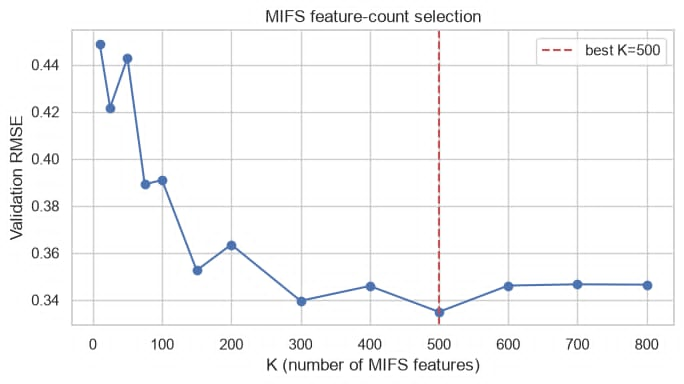
\includegraphics[width=0.75\textwidth]{src/images/mifs_ksweep.jpeg}
\captionsetup{justification=centering}
\caption{K-sweep validation for Method 2 (expanded candidate pool)}
\label{fig:ksweep_method2}
\end{figure}

\textbf{Physical Sanity Check of Selected Features:} A spatial mapping of the 500 retained features confirmed adherence to established ENSO physics. The algorithm autonomously favored data geographically centered on the Ni\~{n}o 3.4 box for Sea Surface Temperatures. Furthermore, Ocean Heat Content (\texttt{sohtc300}) dominated the feature pool (213 of 500 selected features), correctly identifying the deep western Pacific equatorial thermocline as the strongest predictor of anomalous surface changes three months into the future.

\begin{figure}[H]
\centering
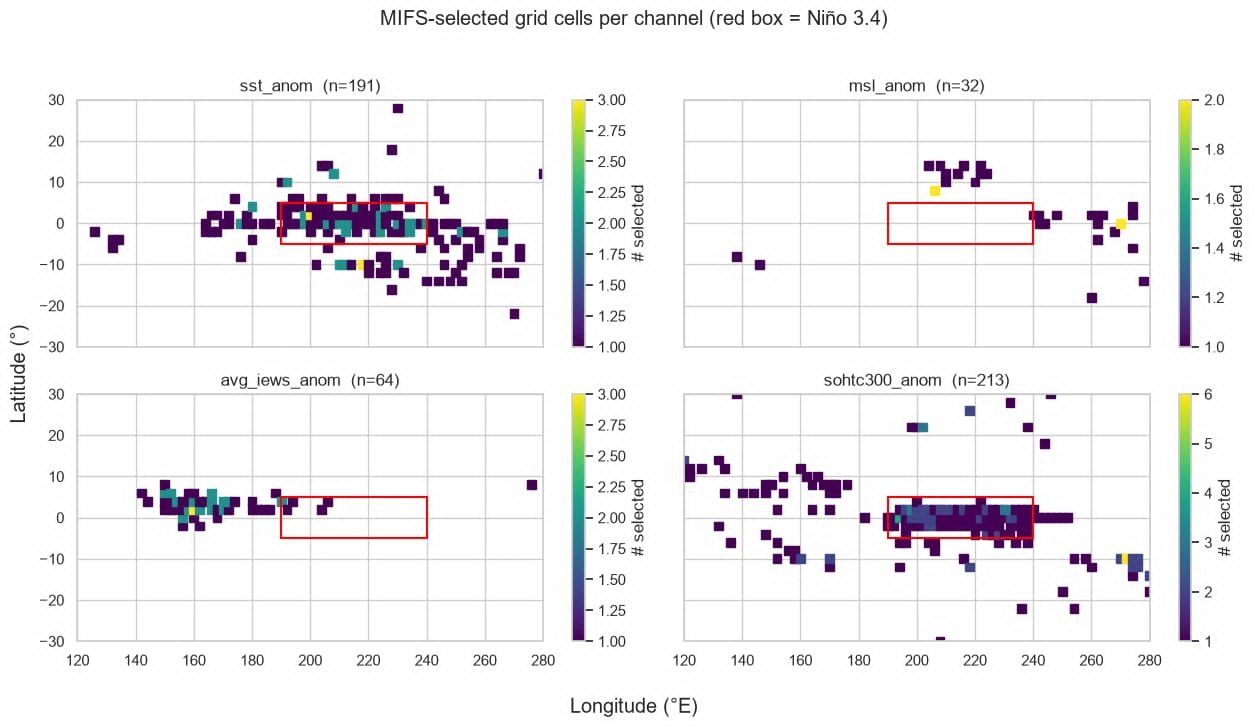
\includegraphics[width=1.0\textwidth]{src/images/mifs_spatial_map.jpeg}
\captionsetup{justification=centering}
\caption{Geographic distribution of the 500 Method-2 MIFS-selected grid cells across the six input channels.}
\label{fig:mifs_map}
\end{figure}

\subsection{Comparison of Method 1 and Method 2}
\label{sec:fs-comparison}

The two methodologies embody opposite ends of the candidate-pool-versus-estimator-exactness trade-off introduced in Section~\ref{sec:fs-overview}. Method 1's restricted, stratified pool of at most 300 candidates keeps the exact k-nearest-neighbour redundancy estimator tractable, and its K-sweep (Figure~\ref{fig:ksweep}) selects a compact feature set an order of magnitude smaller than Method 2's. Method 2's expanded pool of 3,000 candidates, combined with the Gaussian correlation approximation of redundancy, instead settles on a substantially larger feature set of $K=500$, reaching a validation RMSE of $0.3349$ at that point (Figure~\ref{fig:ksweep_method2}). Both methods independently converge on Ocean Heat Content and central-to-eastern equatorial Pacific SST as the dominant contributors to the selected feature set, consistent with established ENSO physics and providing cross-validation of the two search strategies against one another despite their differing candidate pools and redundancy estimators. The downstream baseline modeling implications of this difference in selected feature count are discussed in Section~\ref{sec:xgb-implementation}.

\section{Baseline Model Implementation (XGBoost)}
\label{sec:xgb-implementation}

XGBoost (eXtreme Gradient Boosting) is an ensemble tree model that sequentially adds trees to minimize loss. Both feature-selection methodologies feed into XGBoost baseline models; Method 1 additionally explores a wide regularization grid, while Method 2 uses a single fixed, regularization-aware configuration matched to its larger feature count.

\subsection{Regularization-Focused Grid Search (Method 1)}
To prevent overfitting observed in earlier runs, a regularized grid was designed:

\begin{table}[H]
\centering
\caption{Regularized XGBoost grid (4,374 combinations)}
\label{tab:xgb_grid}
\normalsize
\renewcommand{\arraystretch}{1.2}
\begin{tabular}{|l|l|l|}
\hline
\textbf{Parameter} & \textbf{Baseline} & \textbf{Regularized} \\
\hline
max\_depth & 6 & \textbf{2, 3} \\
\hline
n\_estimators & 500 & 100, 200, 300 \\
\hline
learning\_rate & 0.1 & 0.01, 0.05, 0.1 \\
\hline
subsample & --- & 0.6, 0.7, 0.8 \\
\hline
colsample\_bytree & --- & 0.6, 0.7, 0.8 \\
\hline
min\_child\_weight & --- & 5, 10, 20 \\
\hline
reg\_alpha (L1) & --- & 0, 0.5, 1.0 \\
\hline
reg\_lambda (L2) & --- & 1, 5, 10 \\
\hline
\end{tabular}
\end{table}

\subsection{Baseline XGBoost Formulation}
The baseline architecture acts as a benchmark utilizing the most influential features. The gradient boosting model utilizes specific hyperparameter topologies designed to reduce tree complexity and mitigate the ``curse of dimensionality'' on the flattened tensor:

\begin{table}[H]
\centering
\caption{XGBoost configurations used throughout the K-Sweep and final baseline evaluation.}
\label{tab:xgb_baseline_config}
\normalsize
\renewcommand{\arraystretch}{1.2}
\begin{tabular}{|l|l|}
\hline
\textbf{Parameter} & \textbf{Value} \\
\hline
n\_estimators & 400 \\
\hline
max\_depth & 4 \\
\hline
learning\_rate & 0.05 \\
\hline
subsample & 0.8 \\
\hline
colsample\_bytree & 0.8 \\
\hline
reg\_lambda (L2) & 1.0 \\
\hline
\end{tabular}
\end{table}

This same configuration (\texttt{max\_depth=4}, \texttt{learning\_rate=0.05}, \texttt{reg\_lambda=1.0}, \texttt{subsample=0.8}) was carried forward as the fixed baseline for Method 2, applied directly to the $K=500$ feature set selected via the expanded-pool, Gaussian-approximated MIFS procedure.

\newpage
\subsection{Hyperparameter Tuning Process}

\textbf{Stage 1: Grid Search on Validation Set}
\begin{itemize}
\item Enumerate all parameter combinations ($2 \times 3 \times 3 \times 3 \times 3 \times 3 \times 3 \times 3 = 4374$ combos, max\_depth $\in \{2, 3\}$)
\item Train on train set (457 samples pooled), evaluate on validation set (48 samples)
\item Metric: Validation RMSE
\item Select best hyperparameters: $\theta^* = \arg\min_\theta \text{RMSE}_{\text{val}}(\theta)$
\end{itemize}

\textbf{Stage 2: Final Evaluation on Test Set}
\begin{itemize}
\item Re-train model with $\theta^*$ on train set train+val set (457 samples)
\item Evaluate on held-out test set (35 samples, window end 2023-01 to 2023-12)
\item Metrics: RMSE, ACC (anomaly correlation coefficient)
\end{itemize}

\subsection{Anomaly Correlation Coefficient (ACC)}
For ENSO forecasting, ACC is more operationally relevant than raw RMSE:
\begin{equation}
\text{ACC} = r(y_{\text{true}}, y_{\text{pred}}) = \frac{\text{Cov}(y_{\text{true}}, y_{\text{pred}})}{\sigma_{\text{true}} \cdot \sigma_{\text{pred}}}
\end{equation}
\begin{itemize}
\item Pearson correlation between predicted and actual Ni\~{n}o 3.4 index
\item Range: $[-1, 1]$; higher is better
\item Measures whether model gets the sign and phase correct
\end{itemize}

\textbf{Why ACC Matters for ENSO:}
\begin{itemize}
\item Forecast skill depends on predicting El Ni\~{n}o/La Ni\~{n}a phase correctly
\item A prediction 0.05\degree C off but correct sign $>$ a prediction 0.01\degree C off but wrong sign
\end{itemize}

\section{Deep Learning Model Implementation (CNN-TCN)}
\label{sec:cnn-tcn-implementation}
Section~\ref{sec:cnn-tcn} covers the theoretical methodology for the CNN-TCN architecture. This section covers the implementation details: the specific configuration, hyperparameter choices, and training procedures used to build the model and produce the results in Chapter~\ref{chap:results}. The XGBoost baselines needed explicit feature selection to handle the flattened 216,000-dimensional space; the CNN-TCN instead takes the raw 4D spatio-temporal tensors directly.

\subsection{Framework and Hardware}
The CNN-TCN model was implemented in PyTorch. Training, hyperparameter tuning, and inference all ran on an NVIDIA GPU, needed to accelerate the 2D spatial convolutions and handle the memory load of the 4D input tensors $(12 \times 30 \times 100 \times 6)$.

\subsection{Architectural Hyperparameters}
The network processes the spatial maps independently for each of the 12 monthly snapshots, then models how they evolve over time. The final layer configuration is as follows:

\textbf{Spatial Encoder (CNN):}
\begin{itemize}
    \item \textbf{Input:} $(30 \times 100 \times 6)$ per time step.
    \item \textbf{Convolutional Blocks:} Three blocks of (Conv2d $\rightarrow$ BatchNorm $\rightarrow$ ReLU $\rightarrow$ MaxPool).
    \item \textbf{Feature Maps:} Compresses the complex Pacific grid maps into a rich feature vector of dimension $d=64$.
\end{itemize}

\textbf{Temporal Encoder (TCN):}
\begin{itemize}
    \item \textbf{Input:} Sequence $\mathbf{F} \in \mathbb{R}^{12 \times 64}$.
    \item \textbf{Dilated Causal Convolutions:} Channels set to 64, 32, 32.
    \item \textbf{Hidden Dimension:} The temporal encoder outputs a final context vector.
\end{itemize}

\textbf{Task-Specific Prediction Heads:}
\begin{itemize}
    \item \textbf{ENSO Head (Objective 1):} A dense Multi-Layer Perceptron (MLP) reducing the context vector to a single scalar (Hidden layer size = 64).
    \item \textbf{Impact Head (Objective 2):} Fits a PCA on the training set's [t2m, tp] grids (taking 15 dominant components). The neural network outputs 15 coefficients (via a hidden layer size = 128), which are decoded by a frozen linear PCA layer back into the full South Asian grid.
\end{itemize}

\begin{table}[H]
\centering
\caption{Final CNN-TCN Training Hyperparameters}
\label{tab:cnn_tcn_hyperparams_final}
\renewcommand{\arraystretch}{1.2}
\begin{tabular}{|l|l|}
\hline
\textbf{Hyperparameter} & \textbf{Value} \\
\hline
Optimizer & Adam \\
\hline
Initial Learning Rate & $1 \times 10^{-3}$ \\
\hline
Learning Rate Scheduler & ReduceLROnPlateau (factor=0.5, patience=20) \\
\hline
Batch Size & 8 \\
\hline
Weight Decay (L2) & $1 \times 10^{-4}$ \\
\hline
Dropout Rate & 0.3 \\
\hline
Multi-task Weight ($\alpha$) & 0.5 (ENSO) / 0.5 (Impact) \\
\hline
Spatial Correlation Penalty ($\lambda_{\text{corr}}$) & 0.5 \\
\hline
Early Stopping Patience & 60 epochs \\
\hline
Maximum Epochs & 400 \\
\hline
PCA Components (Impact Head) & 15 \\
\hline
Total Trainable Parameters & $\sim 445,000$ \\
\hline
\end{tabular}
\end{table}

\subsection{Refining and Tuning Process}
Throughout development, several hypotheses were formulated, tested, and iterated upon:
\begin{itemize}
\item \textbf{Precipitation (tp) Asymmetry (Rejected):} A signed log-transform $\text{sign}(x)\log_{10}(1+|x|)$ was tested to handle heavily skewed precipitation anomalies. Evaluation showed this caused a mismatch between the log-space loss and physical-space evaluation, harming spatial correlation (dropped from 0.17 to 0.08). The transform was subsequently rejected and reverted.
\item \textbf{Target Compression (Accepted):} The PCA-15 approach replaced the log-transform, proving to be the optimal mathematical solution for precipitation noise. It achieved the best balance of variance explained ($\sim$62\%) without overfitting.
\item \textbf{Loss Balancing via $\alpha$ (Refined):} The multi-task weighting $\alpha$ was rigorously tested. Tuning $\alpha = 0.6$ (favoring ENSO) collapsed the tp spatial correlation. The ratio was finalized at $\alpha = 0.5$, successfully balancing both the ENSO and local impact tasks.
\end{itemize}

\subsection{PCA Target Compression and Spatial Correlation Loss}
To address the noisy and blurry results observed when predicting 756 individual South Asian grid cells directly, a Principal Component Analysis (PCA) basis was implemented. This forces the model to predict large-scale physical weather patterns rather than isolated pixels. The PCA is fitted on the training set's [t2m, tp] grids, retaining 15 dominant components. The linearity of the PCA decoding perfectly preserves spatial correlations.

Furthermore, standard Mean Squared Error (MSE) loss ignores geography. A custom spatial correlation loss was engineered, mathematically rewarding the model for getting the localized weather pattern correct. The combined loss for the impact head is defined as:
\begin{equation}
\mathcal{L}_{\text{impact}} = \text{MSE} + \lambda_{\text{corr}} \cdot (1 - r_{\text{spatial}})
\end{equation}
where $r_{\text{spatial}}$ is the spatial correlation coefficient and $\lambda_{\text{corr}} = 0.5$.


\subsection{Lead Time Variations and Early Stopping}
Two versions of the CNN-TCN were trained to cover both short-term and extended forecasting, by changing the target alignment during tensor construction (Section~\ref{sec:tensor-construction}):

\begin{itemize}
    \item \textbf{3-Month Lead Model:} Target aligned to $t+3$ months, matching the XGBoost baselines for direct comparison. The training curve (Figure~\ref{fig:cnn_tcn_train_3mo}) shows fast convergence, with the best validation RMSE reached at epoch 4.
    \item \textbf{6-Month Lead Model:} Target aligned to $t+6$ months. Forecasting further out means the temporal encoder has to capture longer-range dependencies, which slows convergence. Best validation RMSE for this configuration came at epoch 46 (Figure~\ref{fig:cnn_tcn_train_6mo}).
\end{itemize}

In both cases, training stopped early if validation RMSE did not improve for 15 consecutive epochs, and the weights from the epoch with the lowest validation RMSE were restored before final testing. This is meant to keep the reported test metrics honest, reflecting how well the model generalizes rather than how well it fits the 2019--2022 validation period -- the same overfitting problem that affected the XGBoost baselines.

\subsection{Multi-Seed Ensemble Architecture}
Climate data evaluation is inherently noisy due to small test-set sizes. Instead of presenting a single training run, the final pipeline utilizes a 5-member ensemble. This brings academic-level statistical rigor (mean $\pm$ standard deviation) to the final reported metrics, ensuring the results reflect the true, stable capability of the model rather than stochastic initialization noise.